
\chapter{Proposed Methodology/Architecture}
\phantomsection

%This is for reference only. Delete before finalization


\begin{center}
    

For every project, the methodology and architecture are very important. In this chapter, the requirements, design, feasibility, and overall plan will be discussed. 
    
\end{center}
%This is for reference only. Delete before finalization



\section{Requirement Analysis \& Design Specification}
\subsection{Requirement Analysis}
 The BC547 transistor and Zener diode are mainly used to create the circuit. The BC547 transistor is particularly used because it works in high-fidelity amplification and minimal signal interference. In this circuit, three different kinds of Zener diodes: 7.5 volts, 10 volts, and 12 volts are used. Six resistors, of two different types, are needed to complete the circuit: 1k ohms and 10k ohms. Working process based on week: \newline
 \textbf{Week 1:}\newline
     \textbf{1. Requirement analysis and circuit design:}\newline
     This involves a close analysis of the project requirements to identify the circuit's scope and functionality. It involves listing the basic circuit design according to the project requirements.\newline
    \textbf{2. Component procurement:}\newline
    After the design of the circuit is finalized, identify all the required components. The components should be high-quality parts sourced in conformation to specifications in the design to ensure no hassle in implementing the circuit.\newline
 \textbf{Week 2:}\newline
    \textbf{1. Circuit simulation and testing on a breadboard:}\newline
    In this stage, the software tools are used to simulate the circuit design to validate it. After successful simulation, the design is assembled on a breadboard, where it is tested for practical performance and any initial issues are identified and resolved.\newline
 \textbf{Week 3:}\newline
    \textbf{1. Prototype refinement and final testing:}\newline
    After receiving the result from the testing with a breadboard, the prototype is refined for further design flaws or inefficiencies. A final version of the prototype will be rigorously tested to confirm that it indeed fits the specifications and works well.\newline
    \newline
    \newline
 \textbf{Week 4:}\newline
    \textbf{1. Documentation and report preparation:}\newline
    In the final stage, everything in the project is documented in detail, be it design processes, testing, or results. A report detailing the project and findings will be prepared for presentation or submission.\newline
\subsection{Design Specification}
\onehalfspacing

 Firstly, a breadboard is needed as a base for the circuit. After that, take the BC547 resistors and place them on the board. Then one side of the 10k ohm resistor is connected to the base pin of the transistor and the other side with the Zener diode. The Zener diode must be placed in reverse order. For the collector pin put the positive side of the LED with the collector pin and the negative side with the 1k ohm resistor. Then connect the emitter pin with the negative side and connect the second side of the 1k ohm resistor with the positive supply source. The black color wire is for identifying the negative connection and the red color wire is for identifying the positive connection of the circuit \cite{b3}. 
\section{Feasibility Study}

\subsection{Overview}
 In this project, Zener diodes are used as a main component, because they give the best outcome in reverse bias. The diode begins to conduct current or voltage when it exceeds the voltage of the knee. Thus, the Zener diode diverts the current that passes through it and works as a stabilizer \cite{b2}. This demonstrates the Zener diode's voltage management capability. The project gives the desired outcome by connecting three Zener diodes in a series connection in a reverse bias. And also connecting the two 9-voltage batteries in a series connection to make an 18-volt battery   \cite{Electronics_Projects_for_Dummies}.
\vspace{.1cm}

\begin{table}[h!]
\centering
\begin{tabular}{|  c  |c|}
\hline
\textbf{      Item      } & \textbf{  Type  }  \\
\hline
Transistor &   BC547   \\
\hline
 Zener Diode  & 7v, 10v, 12v     \\

\hline
 Resistor & 1k ohm  \\
\hline
 Resistor & 10k ohm  \\
\hline
Breadboard  & Big size  \\
\hline
LED Light  & Red, Yellow, Green  \\
\hline
Male to Male Jumper wire  & Black, Red\\

\hline
\end{tabular}
\caption{Using Items }
\end{table}



\subsection{Proposed Methodology}
The purpose of this project is to design and build a voltage level indicator for a 12V battery. The primary purpose is to monitor the charge level of a 12v battery, allowing users to determine the remaining battery life and take appropriate actions such as recharging. If the battery level is higher than or equal to 33\%, the LED light connected to a 7v Zener diode will glow. If the battery level is higher than or equal to 66\%, the LED light connected to a 10v Zener diode will glow. If the battery level is equal to 100\%, the LED light connected to a 12v Zener diode will glow. transistor BC517 which is two transistors integrated into one single component; it was used identically as BC547 in with cascade consisting of two BC547 transistors (right) \cite{2}.


\subsection{Costing }

The table of cost analysis is given in table 2.3.
\begin{table}[h!]
\centering
\begin{tabular}{|  c  |c|c|}
\hline
\textbf{      Item      } & \textbf{  Required piece  } & \textbf{  Price  }  \\
\hline
 BC547 Transistor &  3 pieces & 15 taka    \\
\hline
 Zener Diode  &3 pieces  & 15 Taka    \\

\hline
1k ohm Resistor & 3 pieces & 6 Taka    \\
\hline
10k ohm Resistor & 3 pieces & 21 Taka \\
\hline
Breadboard  & 1 piece & 180 Taka  \\
\hline
LED Light  & 3 pieces & 10 Taka  \\
\hline
9-volt battery & 2 pieces & 150 tk\\
\hline
Male to Male Jumper wire  & 10 pieces & 15 Taka\\
\hline
 & & \textbf{Total cost: 312 Taka}\\
\hline
\end{tabular}
\caption{Cost Analysis }
\end{table}

The alternative Costing table is shown in table 2.3.
\begin{table}[h!]
\centering
\begin{tabular}{|  c  |c|c|c|}
\hline
\textbf{      Item      } & \textbf{  Quantity  } & \textbf{ Unit Price (BDT) } & \textbf{  Total Price (BDT)  }  \\
\hline
 BC547 Transistor &  3  & 5 & 15    \\
\hline
 Resistors &  6 &	1 &	6   \\

\hline
LEDs &	3 &	5 &	15    \\
\hline
Zener Diode	 & 3  &	10 &	30 \\
\hline
Breadboard  & 1 & 180 &180 \\
\hline
Male to Male Jumper wire  & 1 set & 10  & 15 \\
\hline
Battery Clips/Connectors	& 1 &	15 &	15\\
\hline
12-volt battery & 1 & 1000 & 1000\\
\hline
 & &  &\textbf{Total cost: 1275 Taka}\\
\hline

\end{tabular}
\caption{Cost Analysis }
\end{table}
\newline
\newline
\newline
\newline
\newline
\pagebreak
\subsection{System Design}

The circuit design is shown in Figure: 2.1.
\begin{figure}[h!] % 'h' for placing it "here"
    \centering
    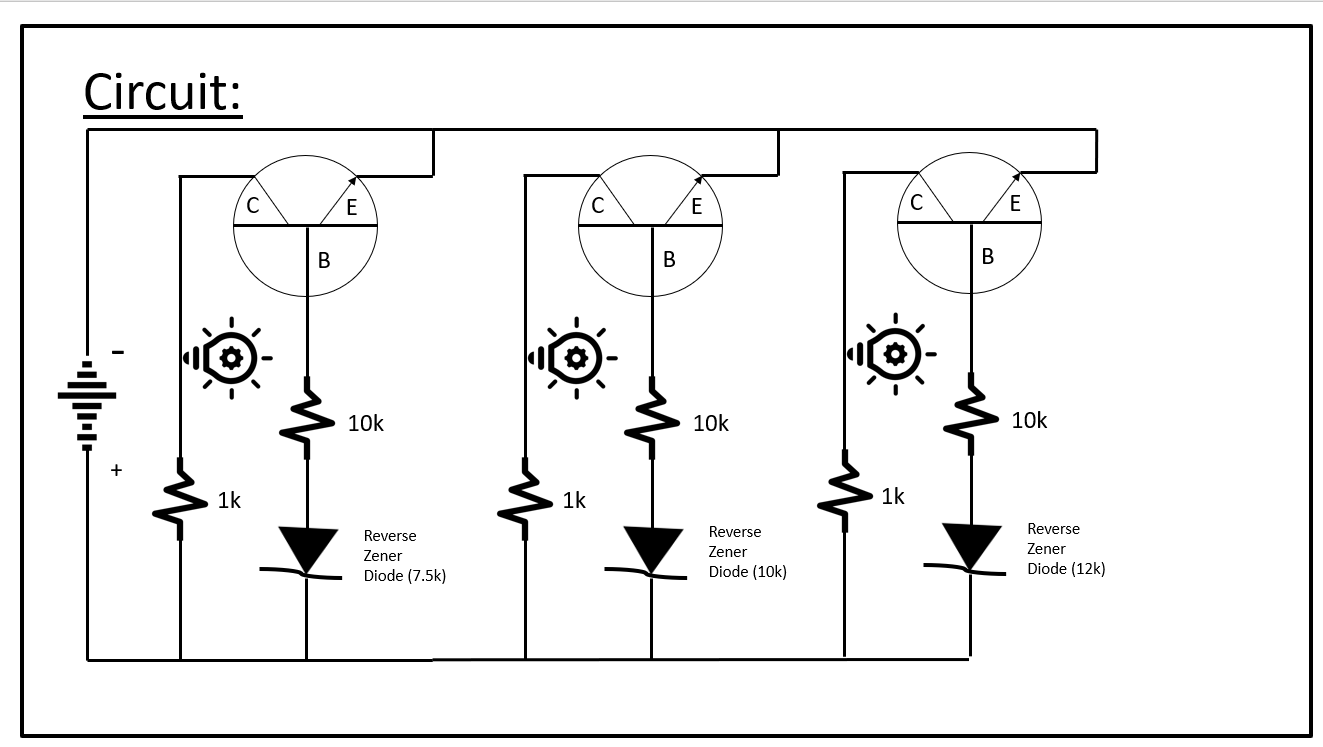
\includegraphics[width=0.5\textwidth]{Diagram.png} % Replace 'diagram.png' with your image file
    \caption{12v Battery Level Indicator}
    \label{fig:sample}
\end{figure}
\subsection{Workflow}
The workflow is shown in Figure: 2.2\newline
\begin{figure}[h] % 'h' for placing it "here"
    \centering
    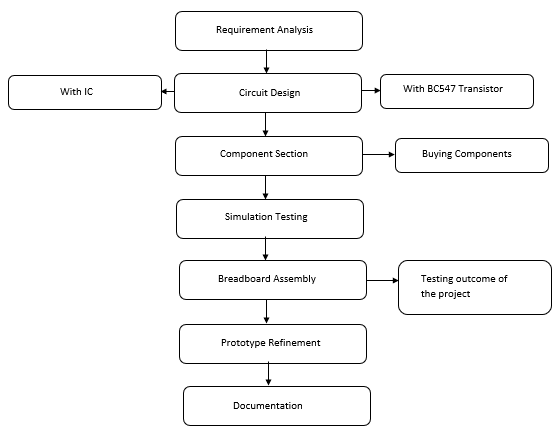
\includegraphics[width=0.5\textwidth]{workflow.png} % Replace 'diagram.png' with your image file
    \caption{Workflow}
    \label{fig:sample}
\end{figure}




\pagebreak
\subsection{Google Site}

\url{https://sites.google.com/diu.edu.bd/batterylevelindicator?usp=sharing}
\newline 
\newline
The circuit design is shown in Figure: 2.3.\newline
\begin{figure}[h!] % 'h' for placing it "here"
    \centering
    
\includegraphics[width=0.5\textwidth]{1.png} % Replace 'diagram.png' with your image file
    \caption{Home Page of Google site}
    \label{fig:sample}
\end{figure}
\newline

The circuit design is shown in Figure: 2.4.\newline
\begin{figure}[h!] % 'h' for placing it "here"
    \centering
    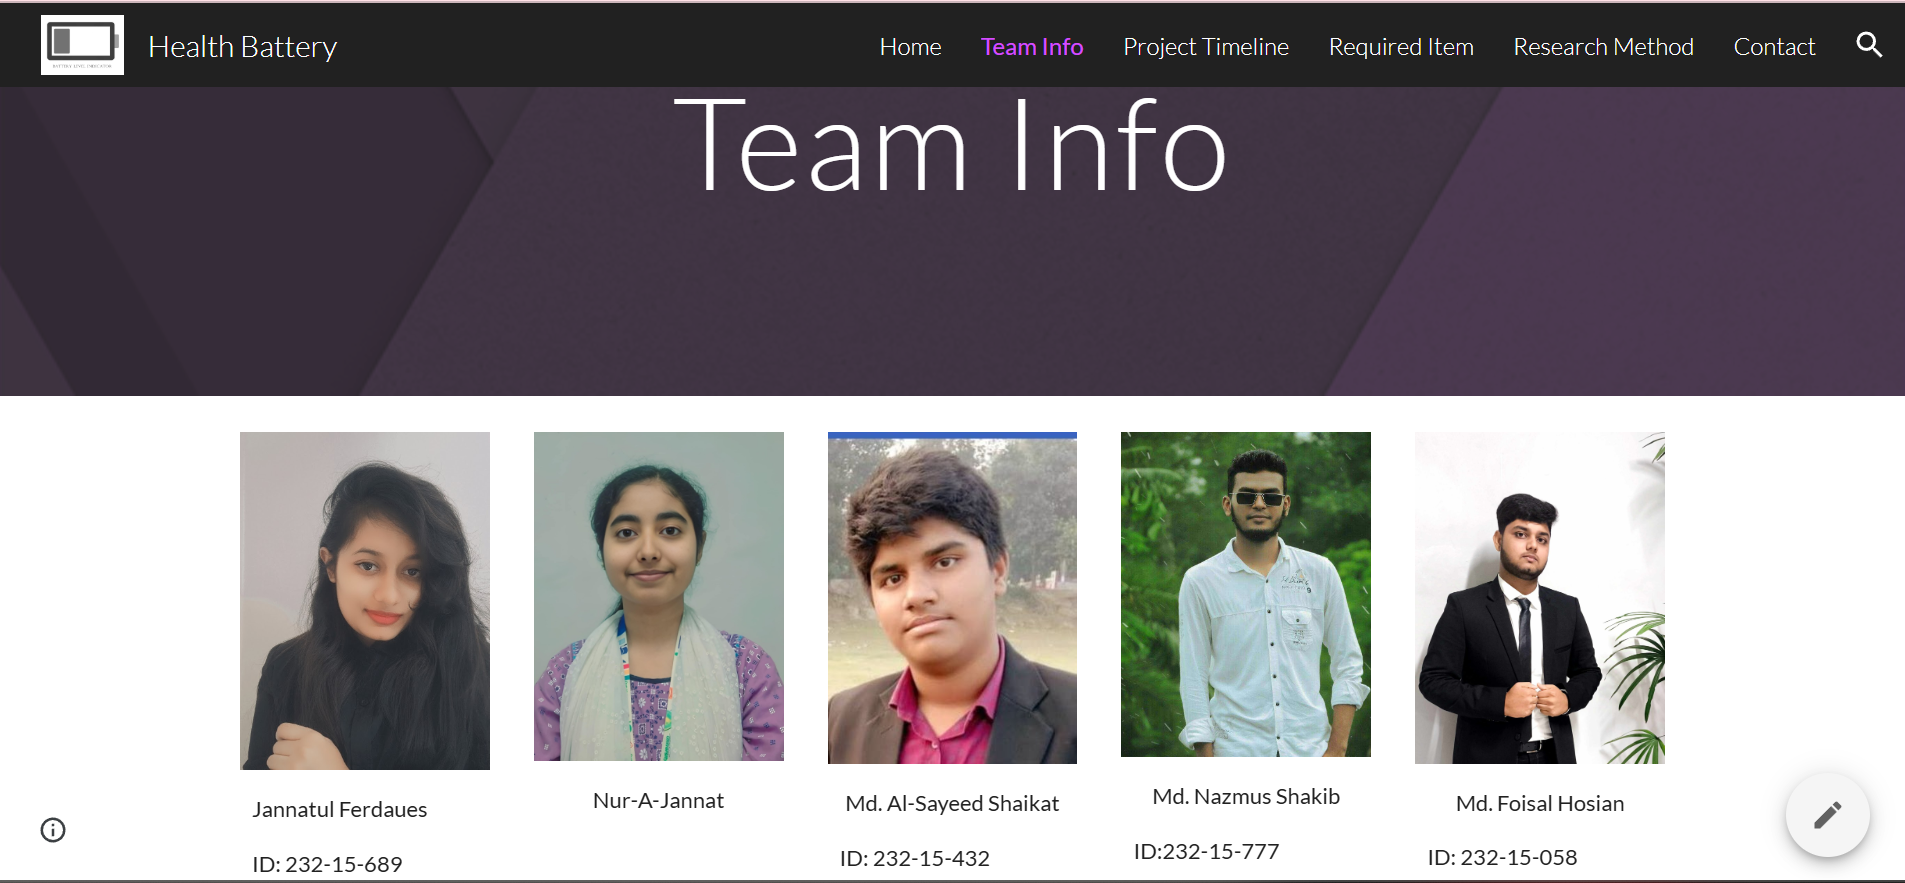
\includegraphics[width=0.5\textwidth]{2.png} % Replace 'diagram.png' with your image file
    \caption{team Info}
    \label{fig:sample}
\end{figure}

\newline The circuit design is shown in Figure: 2.5.
\begin{figure}[h!] % 'h' for placing it "here"
    \centering
    
\includegraphics[width=0.5\textwidth]{3.png} % Replace 'diagram.png' with your image file
    \caption{Time Duration}
    \label{fig:sample}
\end{figure}
\pagebreak
\newline The circuit design is shown in Figure: 2.6.
\begin{figure}[h!] % 'h' for placing it "here"
    \centering
    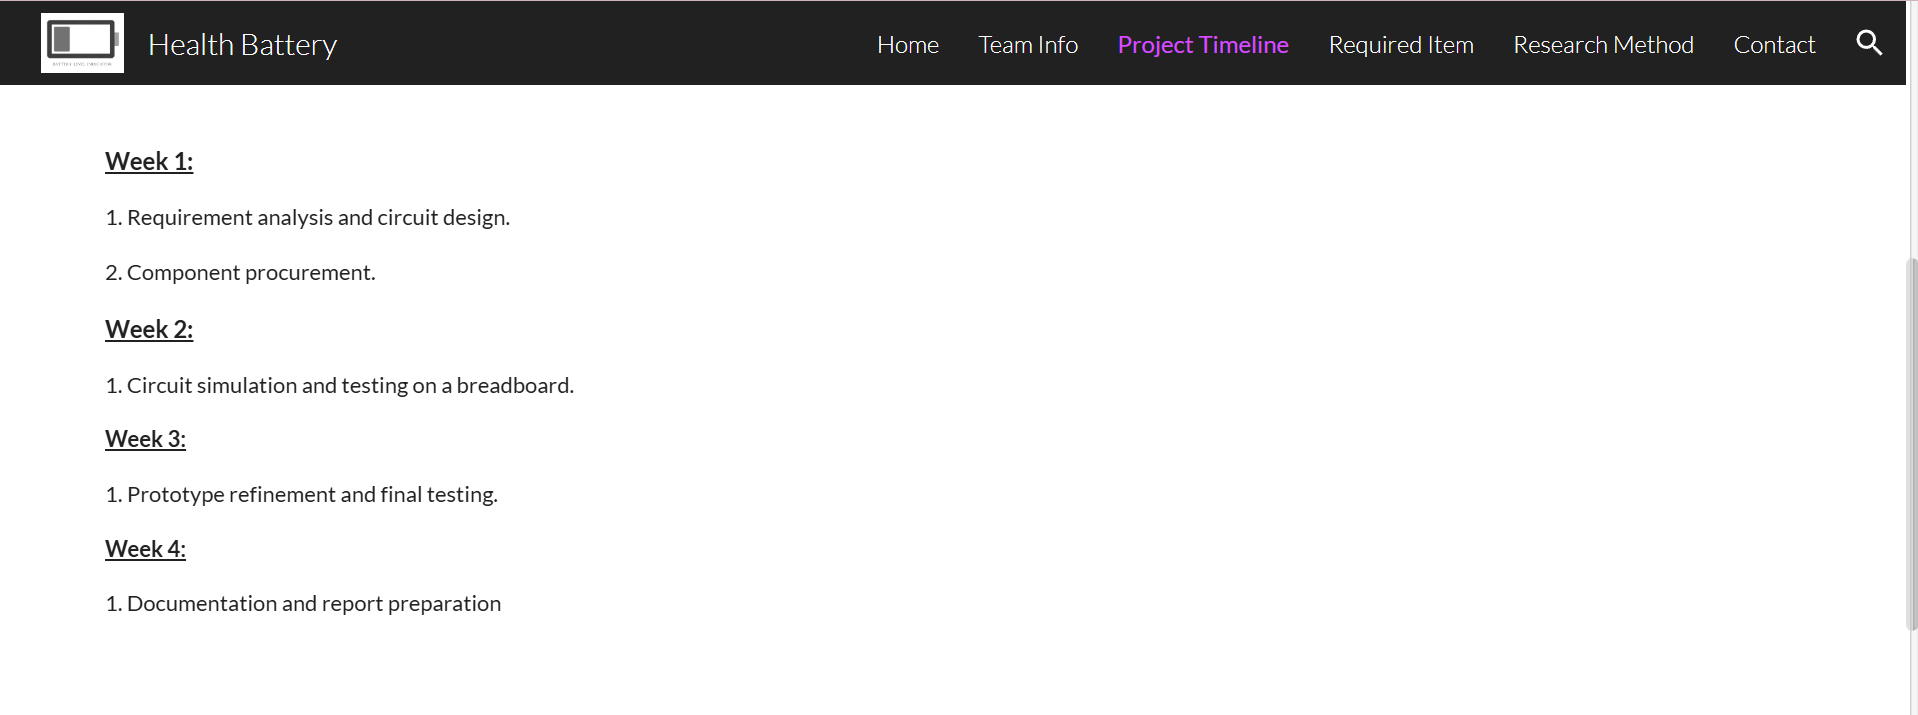
\includegraphics[width=0.5\textwidth]{4.png} % Replace 'diagram.png' with your image file
    \caption{Time Duration( weekly work)}
    \label{fig:sample}
\end{figure}

 \newline The circuit design is shown in Figure: 2.7.
\begin{figure}[h!] % 'h' for placing it "here"
    \centering
    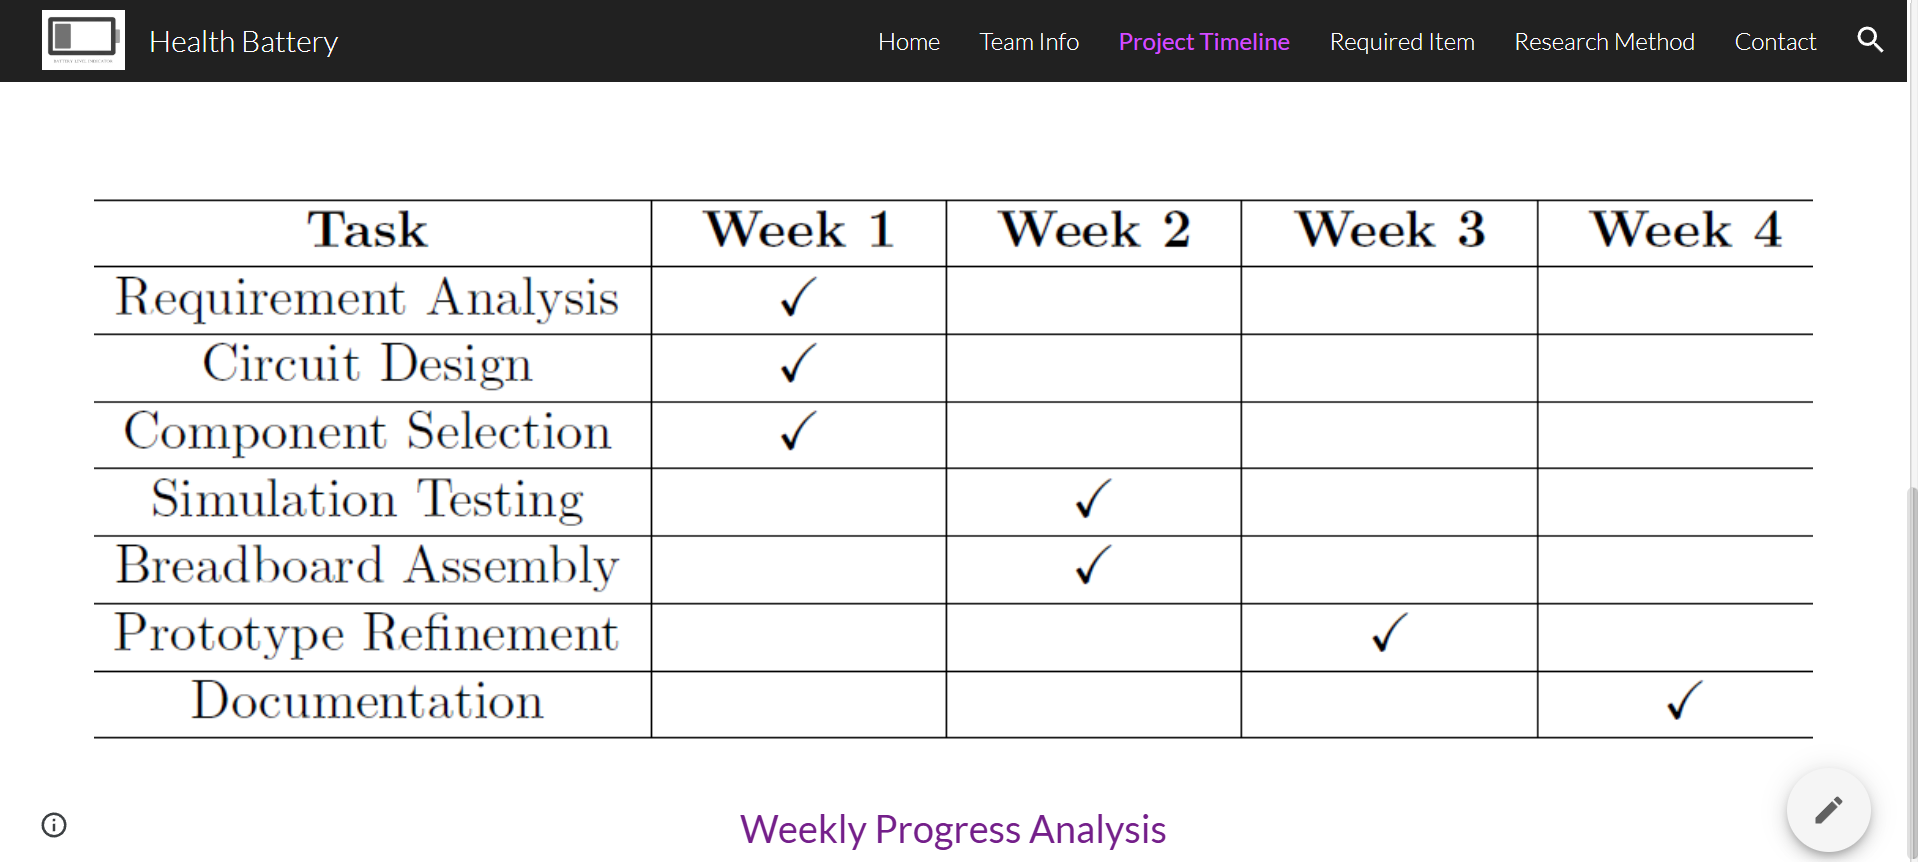
\includegraphics[width=0.5\textwidth]{5.png} % Replace 'diagram.png' with your image file
    \caption{Time Duration analysis}
    \label{fig:sample}
\end{figure}
 \newline The circuit design is shown in Figure: 2.8.
\begin{figure}[h!] % 'h' for placing it "here"
    \centering
    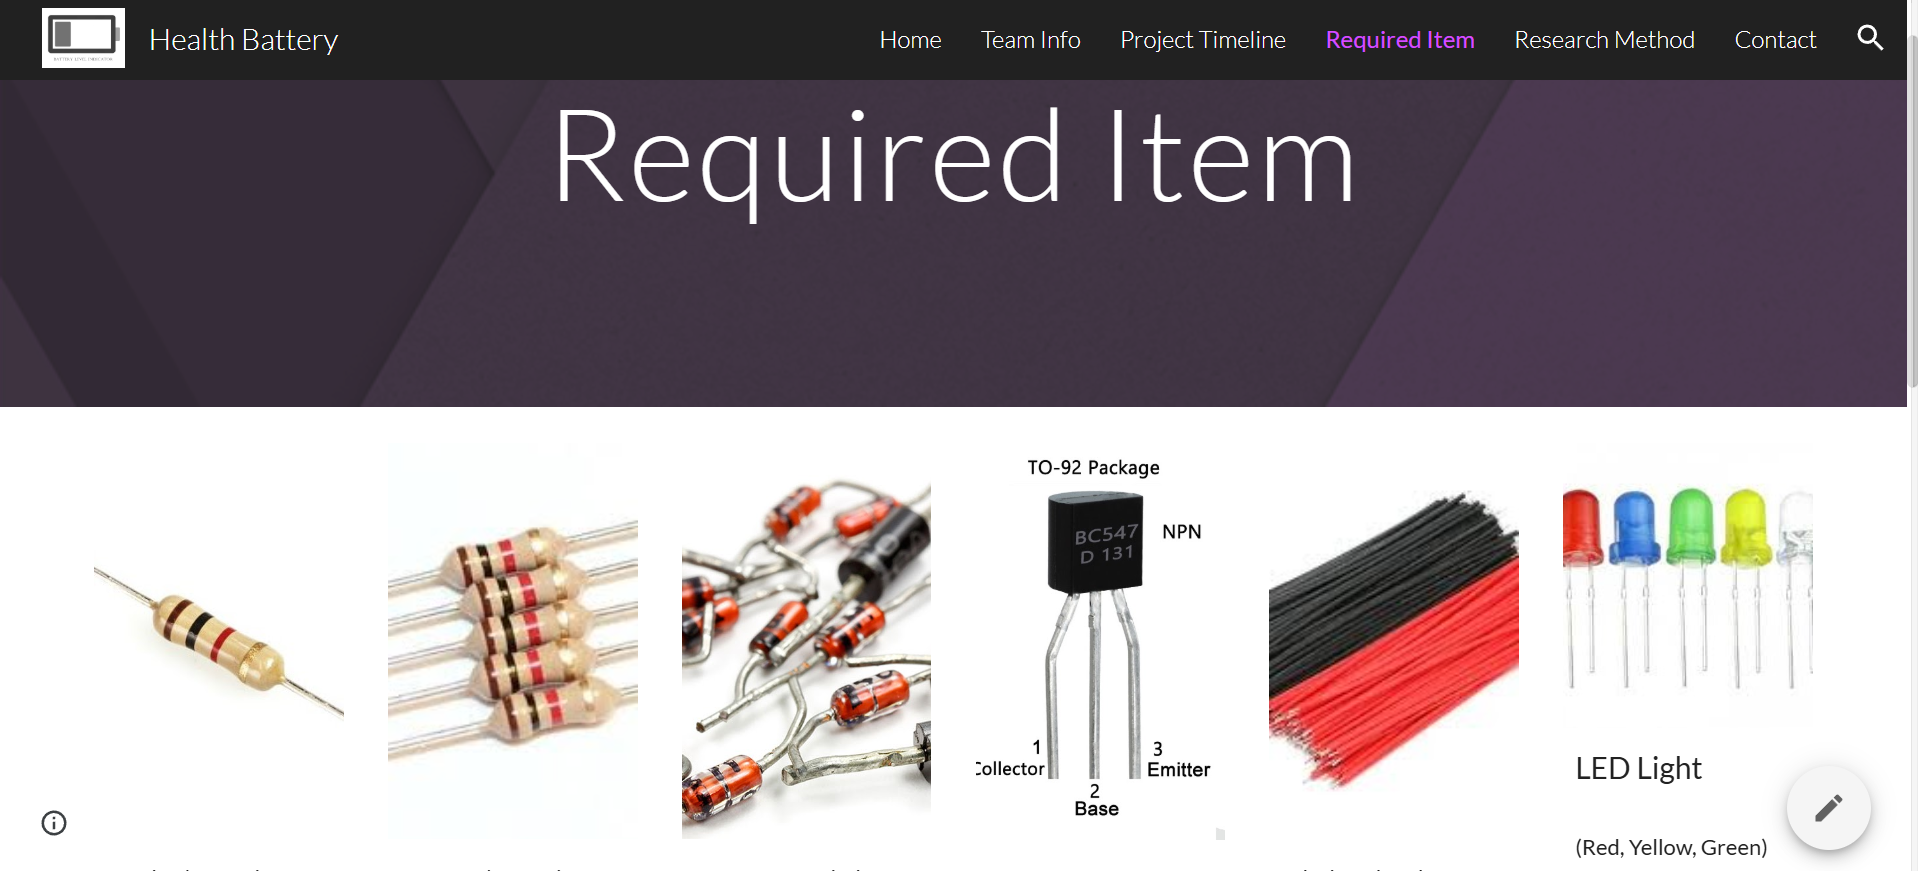
\includegraphics[width=0.5\textwidth]{6.png} % Replace 'diagram.png' with your image file
    \caption{Required Item}
    \label{fig:sample}
\end{figure}
\newline
 \newline The circuit design is shown in Figure: 2.9.
\begin{figure}[h!] % 'h' for placing it "here"
    \centering
    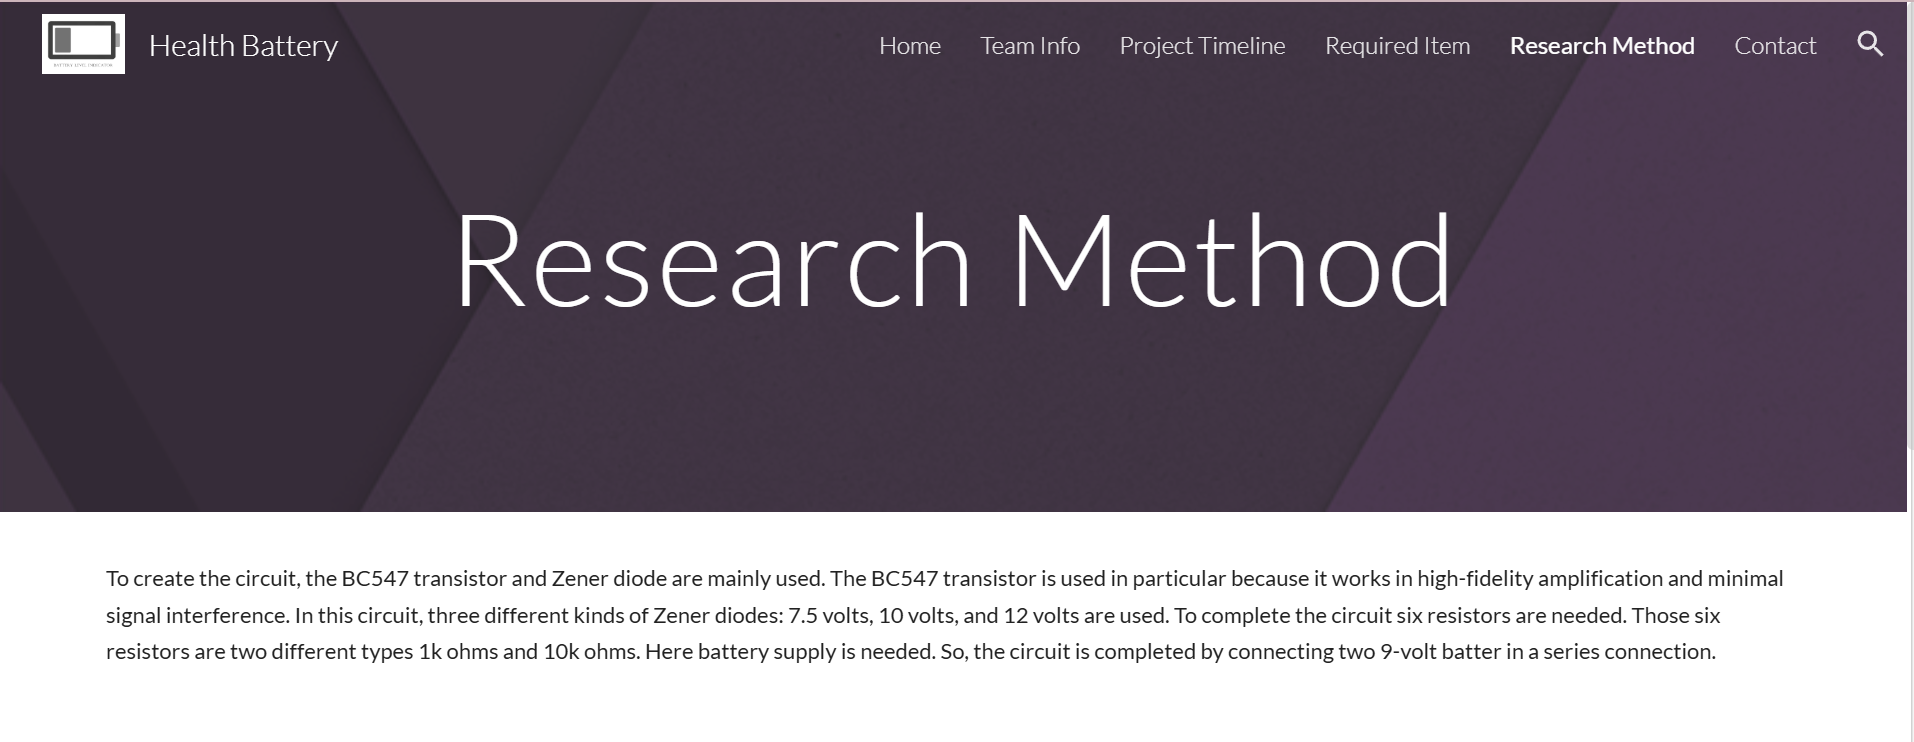
\includegraphics[width=0.5\textwidth]{7.png} % Replace 'diagram.png' with your image file
    \caption{Research Method}
    \label{fig:sample}
\end{figure}
\newline
\pagebreak
 \newline The circuit design is shown in Figure: 2.10.
\begin{figure}[h!] % 'h' for placing it "here"
    \centering
    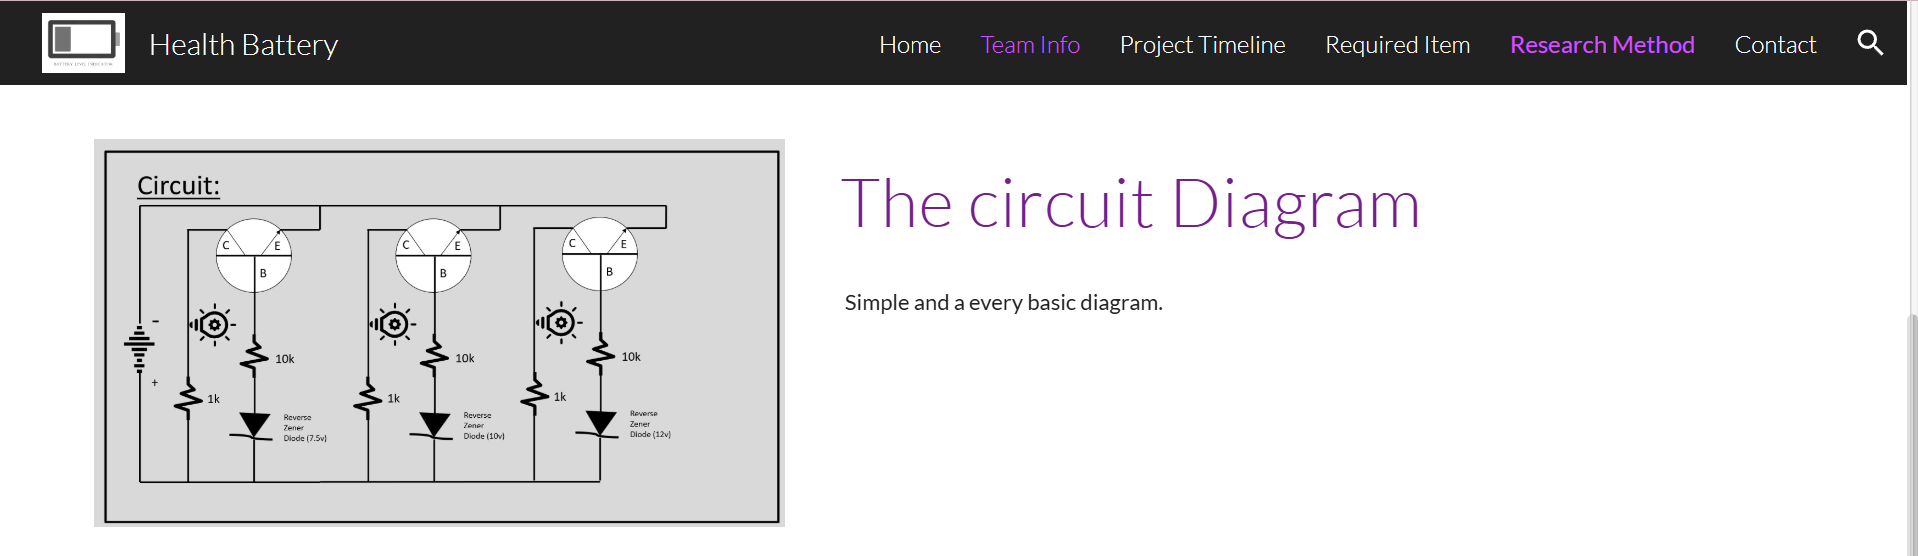
\includegraphics[width=0.5\textwidth]{8.png} % Replace 'diagram.png' with your image file
    \caption{Research Method (circuit diagram)}
    \label{fig:sample}
\end{figure}
 \newline The circuit design is shown in Figure: 2.11.
\begin{figure}[h!] % 'h' for placing it "here"
    \centering
    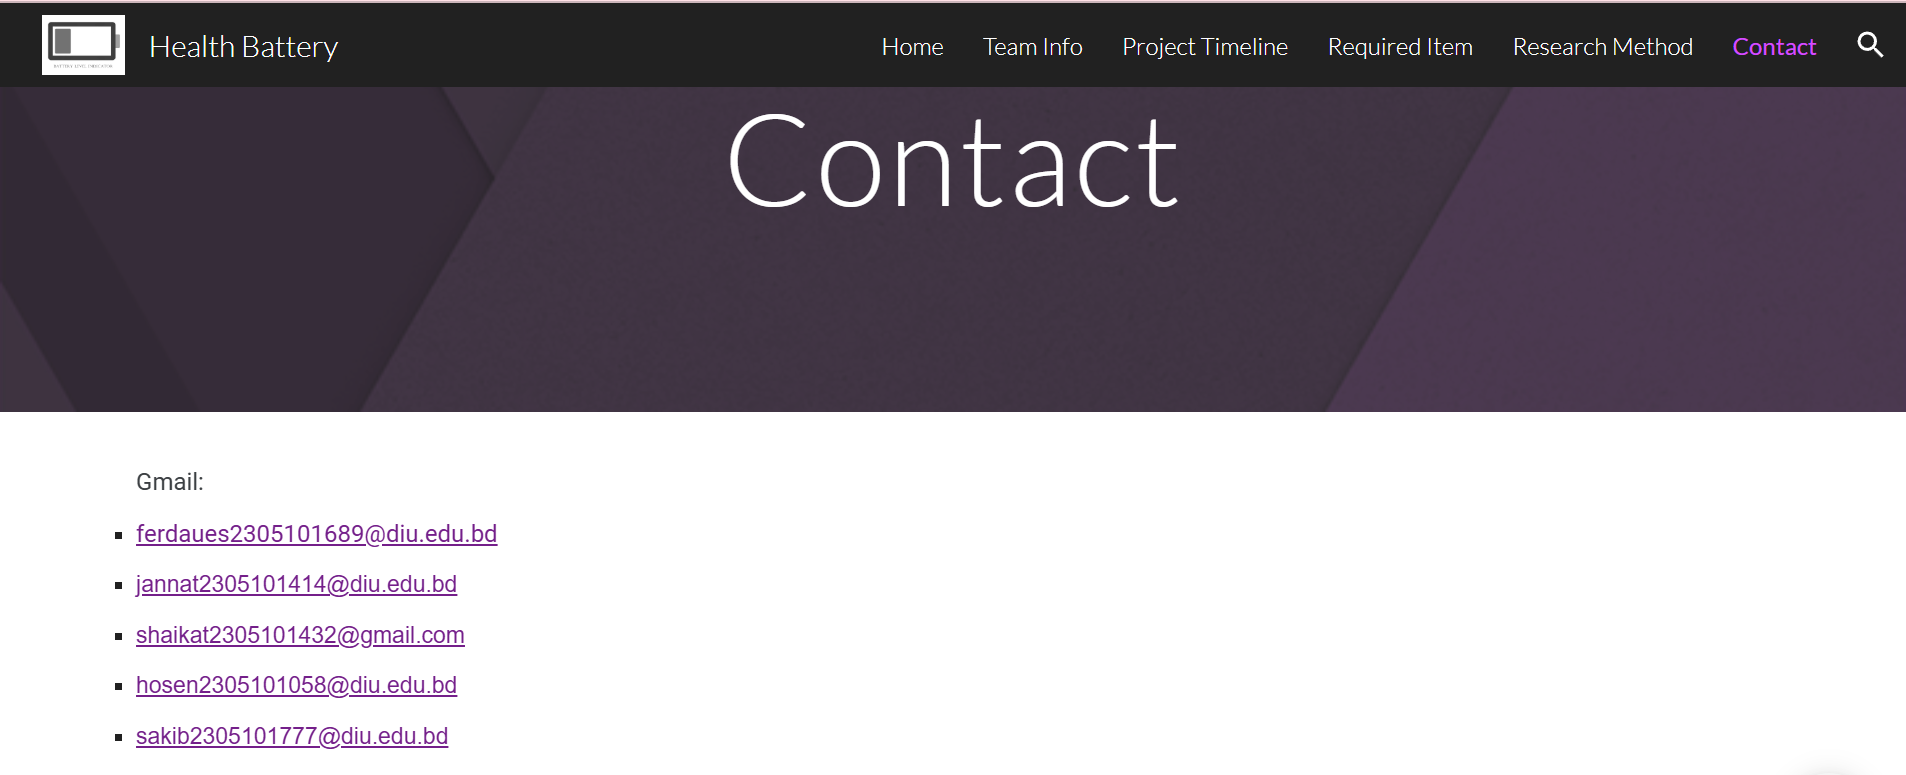
\includegraphics[width=0.5\textwidth]{9.png} % Replace 'diagram.png' with your image file
    \caption{Contact Info}
    \label{fig:sample}
\end{figure}


\section{Overall Project Plan}

The main reason is to create a simple and reasonable project. This can be designed using an IC . In modern-day electronics, rectifiers are used for the conversion of AC to DC voltage. The present investigation focuses on exploring the various rectifier circuits constructed using a transistor(BC547) instead of rectifier diodes (1N4007). Forward and reverse bias conditions of the diode were realized using transistors. Half-wave and full-wave rectifiers were constructed using transistors. The obtained output waveforms were compared with rectifier diode waveforms \cite{3}. 1k ohm resistors are used as current-limiting resistors for LEDs, and 10k ohm resistors are used as base resistors for the transistors. In this project, three different kinds of Zener diodes are used. The 7v Zener diode is used for low-volt detection, the 10v Zener diode is used for medium-range volt detection, and finally, the 12v Zener diode is used for high-voltage detection \cite{b1}.
\vspace{.1cm}

\begin{table}[h!]
\centering
\begin{tabular}{|  c  |c|c|c|c|}
\hline
\textbf{      Task      } & \textbf{  Week 1  } & \textbf{  Week 2  } & \textbf{  Week 3  } & \textbf{  Week 4  } \\
\hline
 Requirement Analysis &  \checkmark &   &   &  \\
\hline
 Circuit Design &  \checkmark &   &   &  \\
\hline
Component Selection & \checkmark &   &   &  \\
\hline
Simulation Testing &  & \checkmark  &   &  \\
\hline
Breadboard Assembly &  &  \checkmark &   & \\
\hline
Prototype Refinement &  &   &  \checkmark &  \\
\hline
Documentation &  &   &   & \checkmark \\
\hline
\end{tabular}
\caption{Weekly Progress Analysis}
\end{table}

\vspace{2cm}
